%%%% SELECT ONE OF THE FOLLOWING COMMANDS %%%%%%%%

%%% TEMPLATE FOR PROCEEDINGS TRACK %%%%
\documentclass[mlabstract]{jmlr}


%%%%%%%%%%%%%%%%%%%%%%%%%%%%%%%%%%%%%%%%%%%%%%%%%

%%%%%%%%%%%%%%%%%%%%%%%%
% Watermark 
%These 4 commands must be removed for the camera-ready version.
\usepackage[hpos=300px,vpos=70px]{draftwatermark}
\SetWatermarkText{\test}
\SetWatermarkScale{1}
\SetWatermarkAngle{0}
%%%%%%%%%%%%%%%%%%%%%%%%%%


   
% The following packages will be automatically loaded:
% amsmath, amssymb, natbib, graphicx, url, algorithm2e


%%% WARNING %%%%
%%% 1) Please, use the packages automatically loaded to manage references, write equations, and include figures and algorithms. The use of different packages could create problems in the generation of the camera-ready version. Please, follow the examples provided in this file.
%%% 2) References must be included in a .bib file.
%%% 3) Write your paper in a single .tex file.
%%%

%%%% SOFTWARE %%%%
%%% Many papers have associated code provided. If that is your case, include a link to the code in the paper as usual and provide a link to the code in the following comment too. We will use the link in the next comment when we generate the proceedings.
%%% Link to code: http://github.com/seancraven/ms_mono

\usepackage{graphicx}
\usepackage{wrapfig}

\usepackage{subcaption}
\usepackage[load-configurations=version-1]{siunitx} % newer version

 % The following command is just for this sample document:
\newcommand{\cs}[1]{\texttt{\char`\\#1}}

 % Define an unnumbered theorem just for this sample document:
\theorembodyfont{\upshape}
\theoremheaderfont{\scshape}
\theorempostheader{:}
\theoremsep{\newline}
\newtheorem*{note}{Note}

%%%% DON'T CHANGE %%%%%%%%%
\jmlrvolume{}
\firstpageno{1}
\editors{List of editors' names}

\jmlryear{2023}
\jmlrworkshop{Symmetry and Geometry in Neural Representations}

%\editor{Editor's name}
%%%%%%%%%%%%%%%%%%%%%%%%%%%



\title[Equivariant Planning]{Equivariant Transition Models for Planning}

\author{\Name{Sean Craven} \Email{sean.craven.22@ucl.ac.uk, sean.craven@advai.co.uk} \\
\Name{Caswell Barry} \Email{caswell.barry@ucl.ac.uk} \\
\Name{Augustine Mavour-Parker} \Email{augustine.mavor-parker.15@ucl.ac.uk} \\
\Name{Matthew Sargent} \Email{matthew.sargent.19@ucl.ac.uk} \\
}
 % \addr Address 2
 %}



\begin{document}

\maketitle

\begin{abstract}
	In this initial investigation, we present a novel method of exploiting the symmetry of a MDP. We perform Dyna-style planning with pre-trained equivariant transition models, and see strong improvements upon non equivariant transition models and agents that don't plan with the same training data and number of parameters. Extending this to learning a transition model is suggested as future work.
\end{abstract}

\section{Introduction}
Encoding equivariance into deep reinforcement learning agent's networks has been an effective inductive bias for reinforcement learning agents in symmetric environments. Enabling agents to learn effective policies with superior sample efficiency \cite{van2020plannable, mondal2020group} or learn policies on previously unapproachable tasks \cite{wang2022so2}. These works exploit properties of group structured MDP homomorphisms~\cite{ravindran2003smdp, ravindran2001symmetries}. Where the symmetry is described by a discrete group $G$. This forms a subset of Markov Decision Process (MDP), where in the deterministic case they obey:
\begin{equation}
	T(S, A) = S', \\
	T(g \cdot S, g \cdot a) = g \cdot S',
	\label{eq:gs_mdp}
\end{equation}
\begin{equation}
	R(S, A) = R(g \cdot S, g \cdot A) = r.
	\label{eq:gs_mdp_rw}
\end{equation}
Here $S, S' \in \mathcal{S}$ are states, and $A \in \mathcal{A}$ is an action. $g \in G$ are group actions acting on the state action space. This definition is taken from \cite{van2020plannable}, with slightly altered notation. These notions can be extended to stochastic MDPs.

Our preliminary findings focus on extending the equivariant inductive bias to a transition model of the environment, to enable planning. Our initial investigation focus around augmenting a Proximal Policy Optimization (PPO)~\cite{schulman2017proximal} agent with the ability to plan using learned transition models.

We implemented a Dyna-style agent, which directly learnt a policy from both the real environment, and trajectories simulated by an equivariant transition model. To achieve this a novel method of polling is proposed to produce approximately equivariant transition models. In our initial testing we see promising potential when planning with equivariant transition models. However, we failed to implement a Dyna-style agent that outperformed a PPO agent in the Cart-Pole\cite{florian2007correct, barto1983neuronlike} and Catch~\cite{osband2020bsuite} environments that were tested in\footnote{Both environment use their default parameters in Gymnax~\cite{lu2022discovered}}.

\section{Method}
The Dyna-style training process for the equivariant agents consists of equal length planning and acting phases. In the acting phase the agent gains experience in the real environment, which is followed by a planning phase. Where the agent gains experience from a simulated MDP. The transition model, $T$, of the simulated MDP is constructed with a Group-Convolutional Neural Network (G-CNN)~\cite{cohen2016group}.

To construct a transition model $T: \mathcal{S} \times \mathcal{A} \rightarrow \mathcal{A}$, maps from state and action space to state space. Where each state has a well-defined shape.

Each group convolution layer is constructed out of a single kernel, the parameters of the network, which is convolved with the input. For each group action $g \in G$, a different cross-correlation is performed where the cross cross-correlation is between the group action acting on the kernel, $k$, and, $f$, the input. Thus, a layer takes the form of,
\begin{equation}
	t(x) = \begin{pmatrix}
		(k \cdot g_0* f )(x)  \\
		(k \cdot g_1 * f )(x) \\
		\vdots                \\
		(k \cdot g_{|G|} * f)(x)
	\end{pmatrix}.
	\label{eq:g-cnn}
\end{equation}
Where $k$ is the kernel cross-correlated with the input $f$. In our setting each cross-correlation produces an output of the same shape as a state. As such, a reduction must be performed to get an output in state space. If a max or average pooling was used over the $|G|$ dimension the equivariance of the group convolution would be lost. The network would become invariant to group operations on the input. This loss of equivariance motivates the need for an equivariant reduction to ensure that the transition models used for planning are fully equivariant.

The proximal pooling layer provides a novel and empirically reliable method to produce equivariant networks. Inspired by the intuition that transitions to subsequent states in many environments are closer to the previous state than a random state sampled from the environment. They layer only requires a distance metric, $d(s, s')$ that measures the difference between two states. In both Catch and Cart-Pole the L1 distance is used between parts of the state.

The forward pass of the network outputs multiple ``transition images", rows of the vector in Equation.\ref{eq:g-cnn}. The objective of the pooling layer is to select the ``transition image", which provides equivariance for the transition model as defined in Equation.\ref{eq:gs_mdp}. If the group action acting upon the input was known beforehand then this could be done analytically, however, this is not always possible. But for the two MDPs tested we found that using a distance metric between $S$, the input state and $S'$, the predicted state was enough to produce fully equivariant network's once trained.

In Cart-Pole, in both untrained and trained networks on 1000 uniformly randomly sampled state the transition models were perfectly accurate and equivariant, when using L1 distance metric between state vectors with 1000 random seeds for network parameters. In catch, on the 675 state action pairs, 1000 randomly seeded untrained networks achieved $98.3 \pm 0.6$ equivariance. Once trained these models again achieved perfect equivariance. With a method for producing equivariant transition models, the question is how well do they work?

\section{Experiments}
Firstly, a set of offline trained world models were produced for each environment. Three different datasets were collected; the first dataset contained a 50/50 split between transition sampled from a expert\footnote{Gymnax's PPO sample agent implementation that reliably completes Cart-Pole episodes with 500 return.} and random policy (joint expert random). The second, contains only actions that move the Pole/Paddle left (left hand), and the final takes only actions sampled from a random policy (random). These random transitions are a disjoint set from the joint expert-random set.

\begin{wrapfigure}{l}{0.6\textwidth}
	\centering
	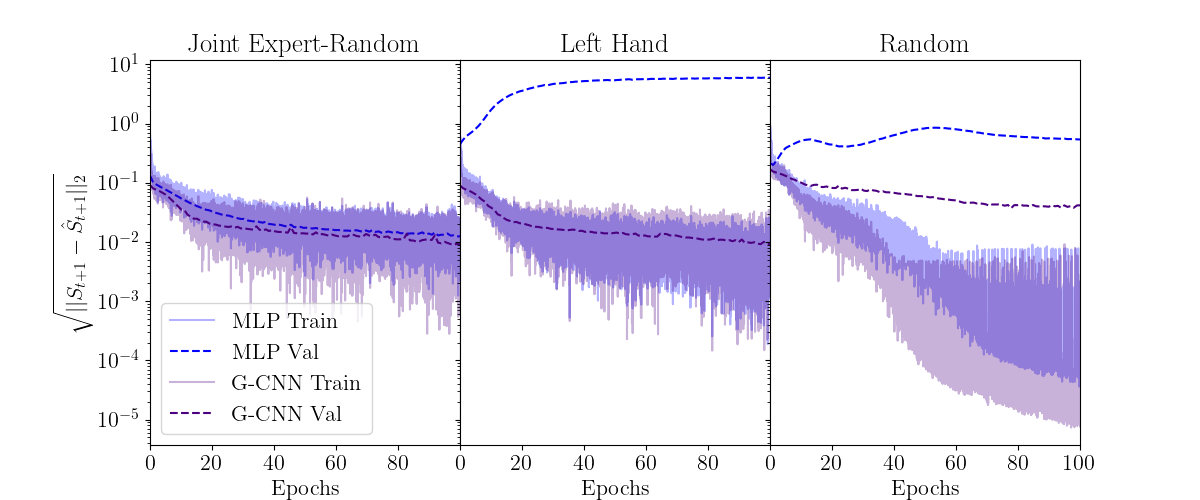
\includegraphics[width=.65\textwidth]{Figures/transition_model_loss.png}
	\caption{Transition Model RMS error, plotted against epochs for three different training
		datasets. Left, the joint expert-random dataset. Center, the same dataset as
		left, however, with only the left action taken. Right, solely transitions sampled
		from a random policy. These datasets contain 400,000 transitions. All plots have
		the same set of validation data with a 50/50 split of expert and random policy
		sampled data.}\label{fig:tm_cp}
\end{wrapfigure}

The training and validation loss for the three equivariant transition models (G-CNNs) are plotted against comparable MLP networks with the same depth and parameter count on these three different datasets. Each dataset contains $400,000$ transitions. In all three figures the model is validated on a new expert policy sampled dataset. This enables testing out of distribution generalisation.

Reassuringly, the effort put into encoding a symmetric inductive bias into the transition model clearly pays off, with in all cases the equivariant transition model outperforming the MLP. In the central plot of Figure~\ref{fig:tm_cp}, the equivariant model generalises very well to transitions that are out of the distribution of the ``left hand" training dataset. This is the key property of the equivariance exploiting the symmetry of the environment, such that if the state is transformed by a group action so is the policy.

Interestingly, the G-CNNs equivariance enables the model to generalise better than the MLP to the expert policy sampled validation set, when trained on a random policy sampled data. This is notable because the steady state distributions of an expert and random policy are vastly different. Empirically, expert policies sample many more transitions at small angles\footnote{See appendix Figure~\ref{fig:cp_hist}}. This is an encouraging result for learning the equivariant transition model online. Where generalising to transitions in small angles for Cart-Pole is important in the early stages of learning. When the policy is improving, but the transition data is mostly random. The story for the Cart-Pole transition model is much the same and is left out for the sake of brevity.

\begin{figure}
	\centering
	\begin{minipage}[b]{.5\textwidth}
		\centering
		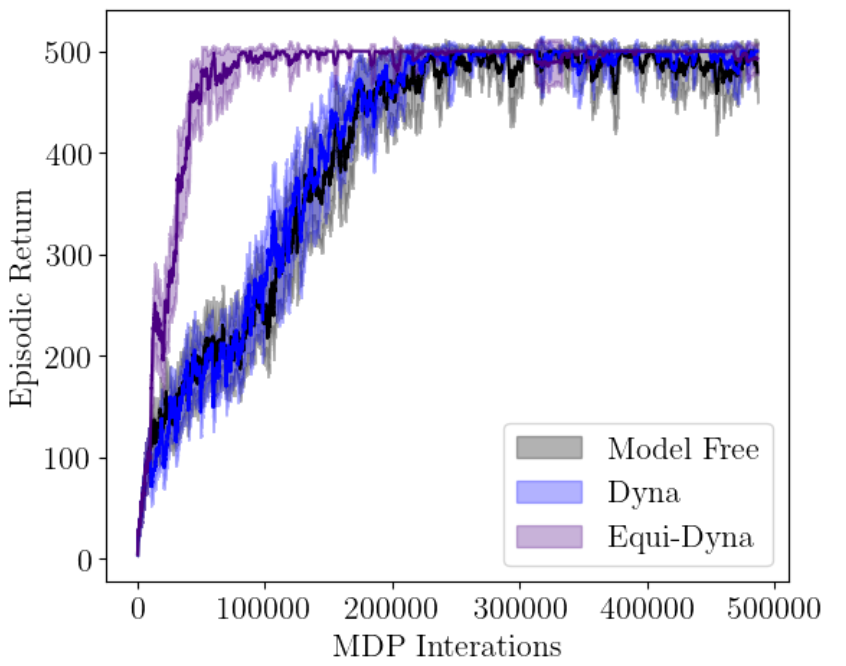
\includegraphics[width=\textwidth]{Figures/best_cp.png}
	\end{minipage}%
	\begin{minipage}[b]{.5\textwidth}
		\centering
		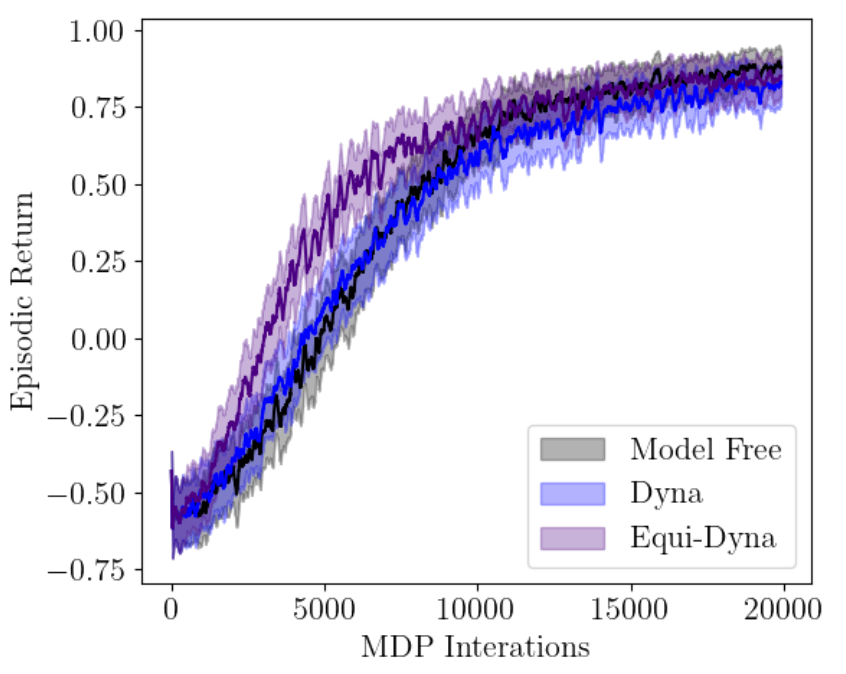
\includegraphics[width=\textwidth]{Figures/best_ctch.png}
	\end{minipage}%
	\caption{Left: Cart-Pole episodic return plotted against MDP interactions. Right: Catch episodic return plotted against MDP interactions. All agents were run across 128 random seeds with 2 standard errors plotted. The best planning ratios are plotted for all agents.}
	\label{fig:joint}
\end{figure}

The next set of experiments were performed with the models trained on joint expert-random datasets. A PPO two layer MLP agent samples experience from the real environment, and then from the pre-trained transition model. This is then iterated over. The ratio between the number of simulated transitions is the ``planning ratio". In Figure~\ref{fig:joint}, the planning ratios are eight and one for Equi-Dyna and Dyna, respectively. In the Catch environment both model based methods used a planning ratio of four.

From, both of the return curves in Figure~\ref{fig:joint} we see that the equivariant planning models do successfully improve the interaction efficiency of the agents. Further, they substantially improve upon the model's without an inductive bias for the symmetry of the environment. This is a reassuring initial result, that confirms that the proximal pooling layer is an effective method to implement approximate equivariance in transition models.

\section{Future Work}
Balancing the sample hunger of the transition models while learning them online is quite challenging. In our initial tests, when learning the models online none of the transition models were able to predict accurate enough transitions to plan multiple episodes for agents. This may  in itself not be a problem, learning to plan short term, could prove more fruitful.

In addition, exploring other model based planning algorithms which may be more forgiving to model accuracy may also be a promising avenue for further work.

\newpage

\acks{Acknowledgements go here.}

\bibliography{pmlr-sample}

\appendix
\section{Cart-Pole}
\begin{figure}[H]
	\centering
	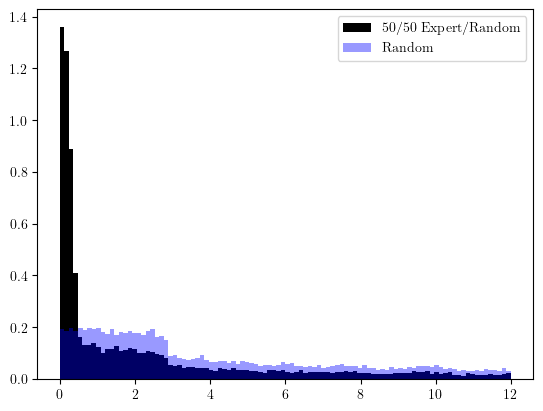
\includegraphics[width=0.95\textwidth]{Figures/angles_cp.png}
	\caption{Histogram of transitions by start angle in Cart-pole, sampled from the joint expert-random dataset and the random dataset}\label{fig:cp_hist}
\end{figure}



\section{Second Appendix}\label{apd:second}


\end{document}

